\documentclass[11pt]{article}

\usepackage[margin=0.85in]{geometry}
\usepackage[T1]{fontenc}
\usepackage[utf8]{inputenc}
\usepackage{lmodern}
\usepackage{microtype}
\usepackage{amsmath, amssymb}
\usepackage{booktabs}
\usepackage{array}
\usepackage{xcolor}
\usepackage{graphicx}
\usepackage{caption}
\usepackage{subcaption}
\usepackage{hyperref}
\usepackage{enumitem}
\usepackage{longtable}

\hypersetup{colorlinks=true, linkcolor=blue!60!black, urlcolor=blue!60!black}
\setlist[itemize]{leftmargin=1.4em, itemsep=0.2em, topsep=0.3em}

\definecolor{lora}{RGB}{29,57,196}
\definecolor{fft}{RGB}{212,107,8}
\definecolor{green}{RGB}{56,158,13}

\title{\textbf{LoRA Geometry and Mixture-of-Experts Results}\\
\large Presentation-Ready Figures, Tables, and Analysis}
\author{}
\date{RoBERTa-base $\cdot$ GLUE (SST-2, MRPC, RTE, MNLI, QNLI, QQP)}

\begin{document}
\maketitle
\tableofcontents
\vspace{1em}

% -----------------------------------------------------------------------
\section{Experimental Setup}
\label{sec:setup}
% -----------------------------------------------------------------------

\subsection*{Models and Tasks}

\begin{center}
\begin{tabular}{lll}
\toprule
\textbf{Role} & \textbf{Model} & \textbf{Tasks} \\
\midrule
Base model & \texttt{roberta-base} & All \\
LoRA adapters & \texttt{rambodazimi/roberta-base-finetuned-LoRA-\{TASK\}} & SST-2, MRPC, RTE, MNLI, QNLI, QQP \\
Full FT & \texttt{rambodazimi/roberta-base-finetuned-FFT-\{TASK\}} & SST-2, MRPC, RTE, MNLI, QNLI, QQP \\
\bottomrule
\end{tabular}
\end{center}

\subsection*{Evaluation Protocol}

\begin{itemize}
\item Validation-split evaluation: up to 2{,}000 examples per task (full split for SST-2/MRPC/RTE).
\item Primary metric: accuracy for single-label tasks; $(\text{acc}+F_1)/2$ for MRPC and QQP.
\item Three evaluation \emph{tracks}: oracle-routed LoRA MoE, per-task LoRA (standalone), per-task FFT.
\item Geometry analysis: SVD of $\Delta W = W_\mathrm{FT} - W_0$ and $\Delta W_\mathrm{LoRA} = W_\mathrm{LoRA} - W_0$ on all 24 query/value attention matrices (12 layers $\times$ $\{W_q, W_v\}$).
\end{itemize}

% -----------------------------------------------------------------------
\section{Spectral Energy of Full Fine-Tuning Updates}
\label{sec:svd}
% -----------------------------------------------------------------------

\subsection*{What the Plot Shows}

We compute the cumulative spectral energy of the weight update $\Delta W_\mathrm{FT}$ for every query and value attention matrix in RoBERTa-base fine-tuned on SST-2:
\[
E(k) = \frac{\sum_{i=1}^{k} \sigma_i^2}{\sum_i \sigma_i^2}.
\]
Each faint blue line is one matrix; the dark curve is the mean.

\begin{figure}[h]
\centering
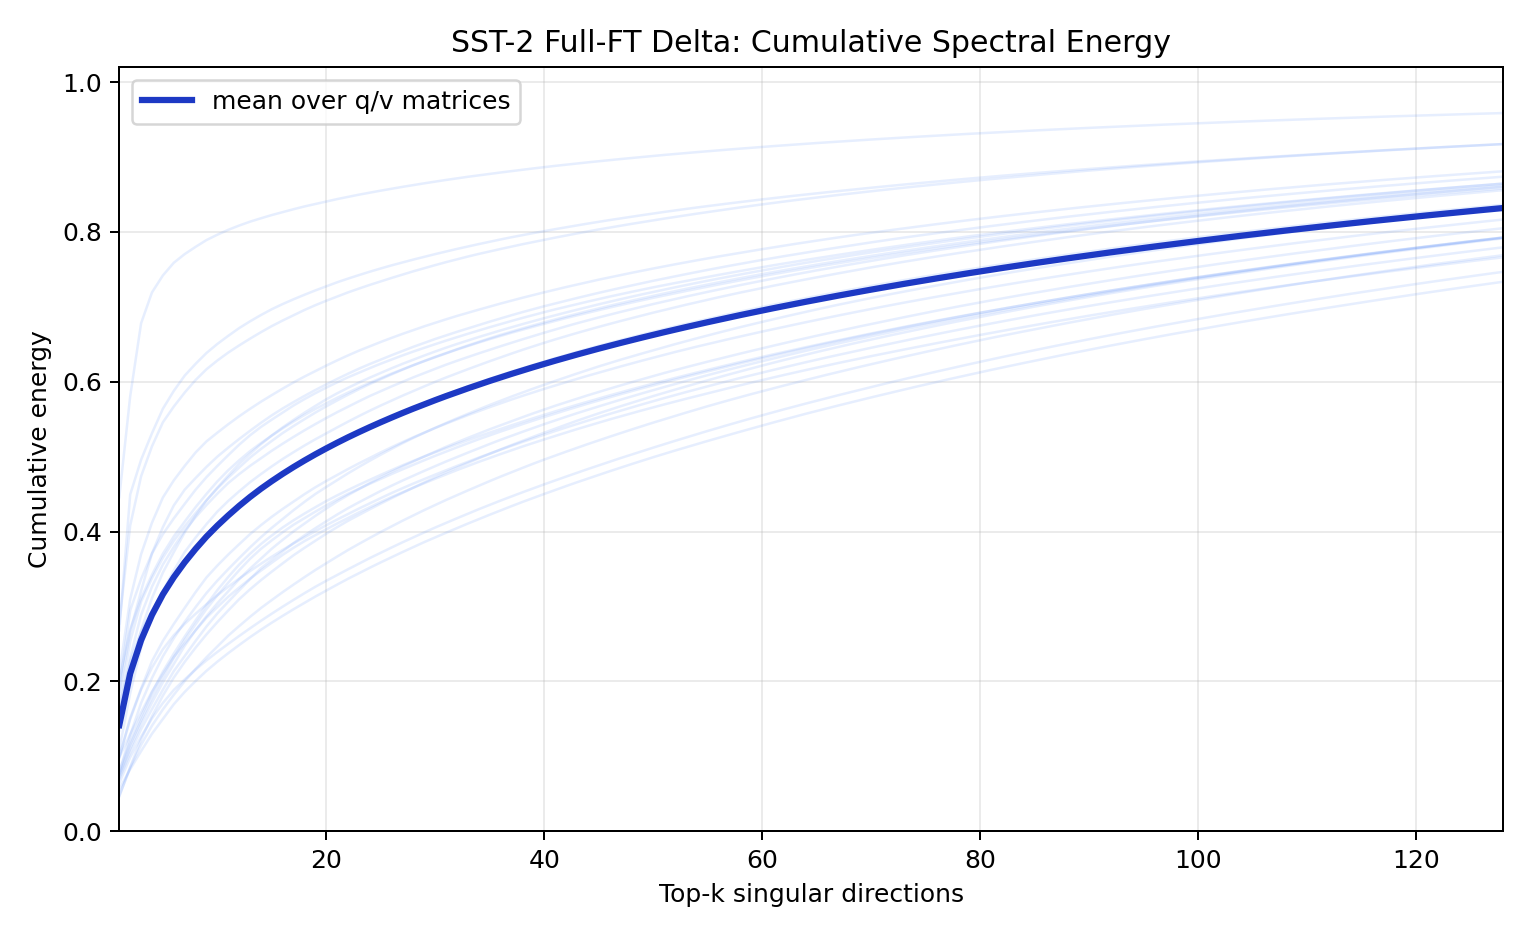
\includegraphics[width=0.82\textwidth]{../figures/sst2_svd_energy.png}
\caption{Cumulative spectral energy of SST-2 full fine-tuning deltas across all 24 attention
query/value matrices. The mean (dark blue) reaches $\approx$50\% of total energy within the top 30
singular directions out of 768. This concentrated structure motivates the LoRA hypothesis: a
low-rank update can capture the most task-relevant directions.}
\label{fig:svd}
\end{figure}

\subsection*{Key Reading}

\begin{itemize}
\item Top-10 directions capture $\approx$40\% of total update energy.
\item Top-40 directions capture $\approx$63\% of total update energy.
\item Full-rank (768 directions) needed for $\approx$100\%.
\item Update is concentrated but not extremely low-rank---consistent with LoRA using rank $r=8$.
\end{itemize}

% -----------------------------------------------------------------------
\section{Subspace Overlap: LoRA vs.\ Full Fine-Tuning}
\label{sec:overlap}
% -----------------------------------------------------------------------

\subsection*{What the Plot Shows}

We compare the top-$k$ left singular subspaces of $\Delta W_\mathrm{FT}$ and $\Delta W_\mathrm{LoRA}$ using:
\[
\phi(k) = \frac{\|U_\mathrm{FT,1:k}^{\top} U_\mathrm{LoRA,1:k}\|_F^2}{k}.
\]
A value of $\phi(k)=1$ means the subspaces are identical; $\phi(k) = k/d$ is the expected value for random independent subspaces ($d=768$).

\begin{figure}[h]
\centering
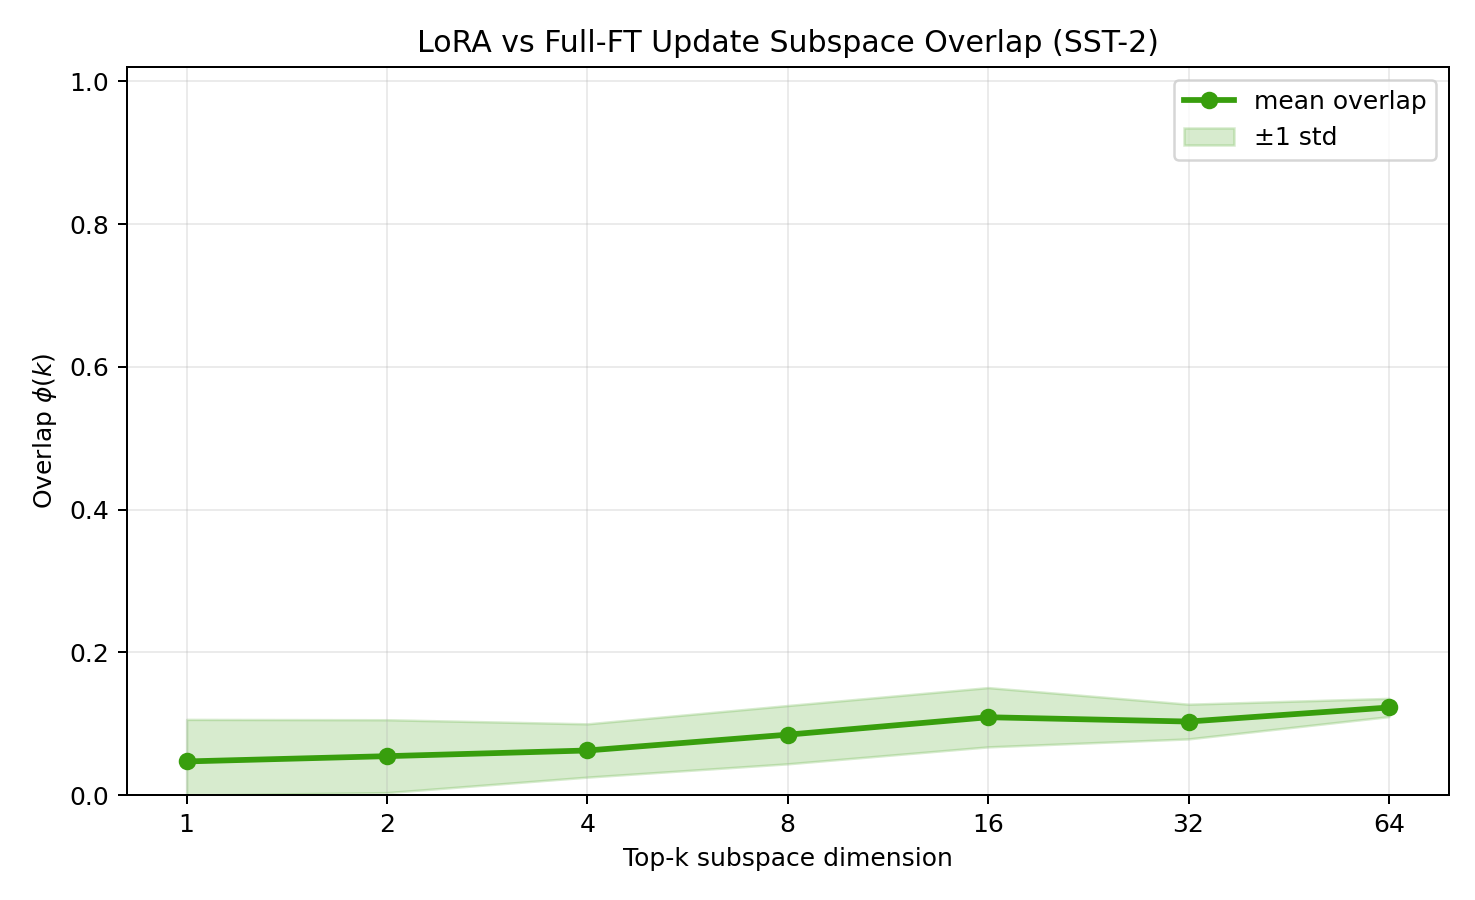
\includegraphics[width=0.78\textwidth]{../figures/sst2_lora_ft_overlap.png}
\caption{Mean subspace overlap $\phi(k)$ between LoRA checkpoint delta and full fine-tuning delta
(SST-2). Error band: $\pm$1 std across 24 query/value matrices. Overlap is above the random-subspace
baseline ($k/d$) at every $k$, with the strongest enrichment at $k=1$ (the single top update
direction is $\approx$38$\times$ above random), confirming that LoRA's update is geometrically
related to full fine-tuning even when using the merged checkpoint as a proxy delta.}
\label{fig:overlap}
\end{figure}

\subsection*{Subspace Overlap Numeric Table}

% Subspace overlap phi(k) between LoRA checkpoint delta and Full-FT delta (SST-2, RoBERTa-base)
% phi(k) = ||U_FT[:,0:k]^T U_LoRA[:,0:k]||_F^2 / k
% Exact values from codex_presentation_results/data/overlap_svd_metrics.json
% Computed over all 24 attention query/value matrices (12 layers x {W_q, W_v})
% Random baseline: k/d where d=768
\begin{tabular}{rrrrrr}
\toprule
\textbf{$k$} & \textbf{Mean $\phi(k)$} & \textbf{Std $\phi(k)$} & \textbf{Max $\phi(k)$} & \textbf{Random ($k/d$)} & \textbf{Ratio} \\
\midrule
 1 & 0.0472 & 0.0589 & 0.259 & 0.0013 & $36\times$ \\
 2 & 0.0546 & 0.0510 & 0.203 & 0.0026 & $21\times$ \\
 4 & 0.0625 & 0.0373 & 0.164 & 0.0052 & $12\times$ \\
 8 & 0.0847 & 0.0408 & 0.193 & 0.0104 & $8\times$ \\
16 & 0.1091 & 0.0415 & 0.184 & 0.0208 & $5\times$ \\
32 & 0.1031 & 0.0243 & 0.145 & 0.0417 & $2.5\times$ \\
64 & \textbf{0.1228} & 0.0128 & 0.143 & 0.0833 & $1.5\times$ \\
\bottomrule
\end{tabular}
\vspace{0.4em}

\noindent\small $d=768$ (RoBERTa-base). The single top update direction ($k=1$) is 36$\times$ more
aligned with the full-FT direction than random chance. At $k=64$, overlap is 1.5$\times$ random ---
LoRA spreads over fewer directions than full FT, so enrichment shrinks as $k$ grows.


\vspace{0.5em}

\subsection*{Interpretation}

\begin{itemize}
\item LoRA and full FT do \emph{not} learn the same subspace (max overlap $\approx$13\%), but they are significantly more aligned than random ($\phi$ is 2--38$\times$ the random baseline).
\item The overlap is highest at small $k$, meaning the single most-important update direction is the most shared.
\item As $k$ grows, the enrichment shrinks: LoRA uses only $r=8$ dimensions, while full FT spreads update energy across many directions.
\end{itemize}

% -----------------------------------------------------------------------
\section{Per-Task Performance: Oracle LoRA MoE vs.\ LoRA vs.\ FFT}
\label{sec:pertask}
% -----------------------------------------------------------------------

\subsection*{What the Figure Shows}

\begin{figure}[h]
\centering
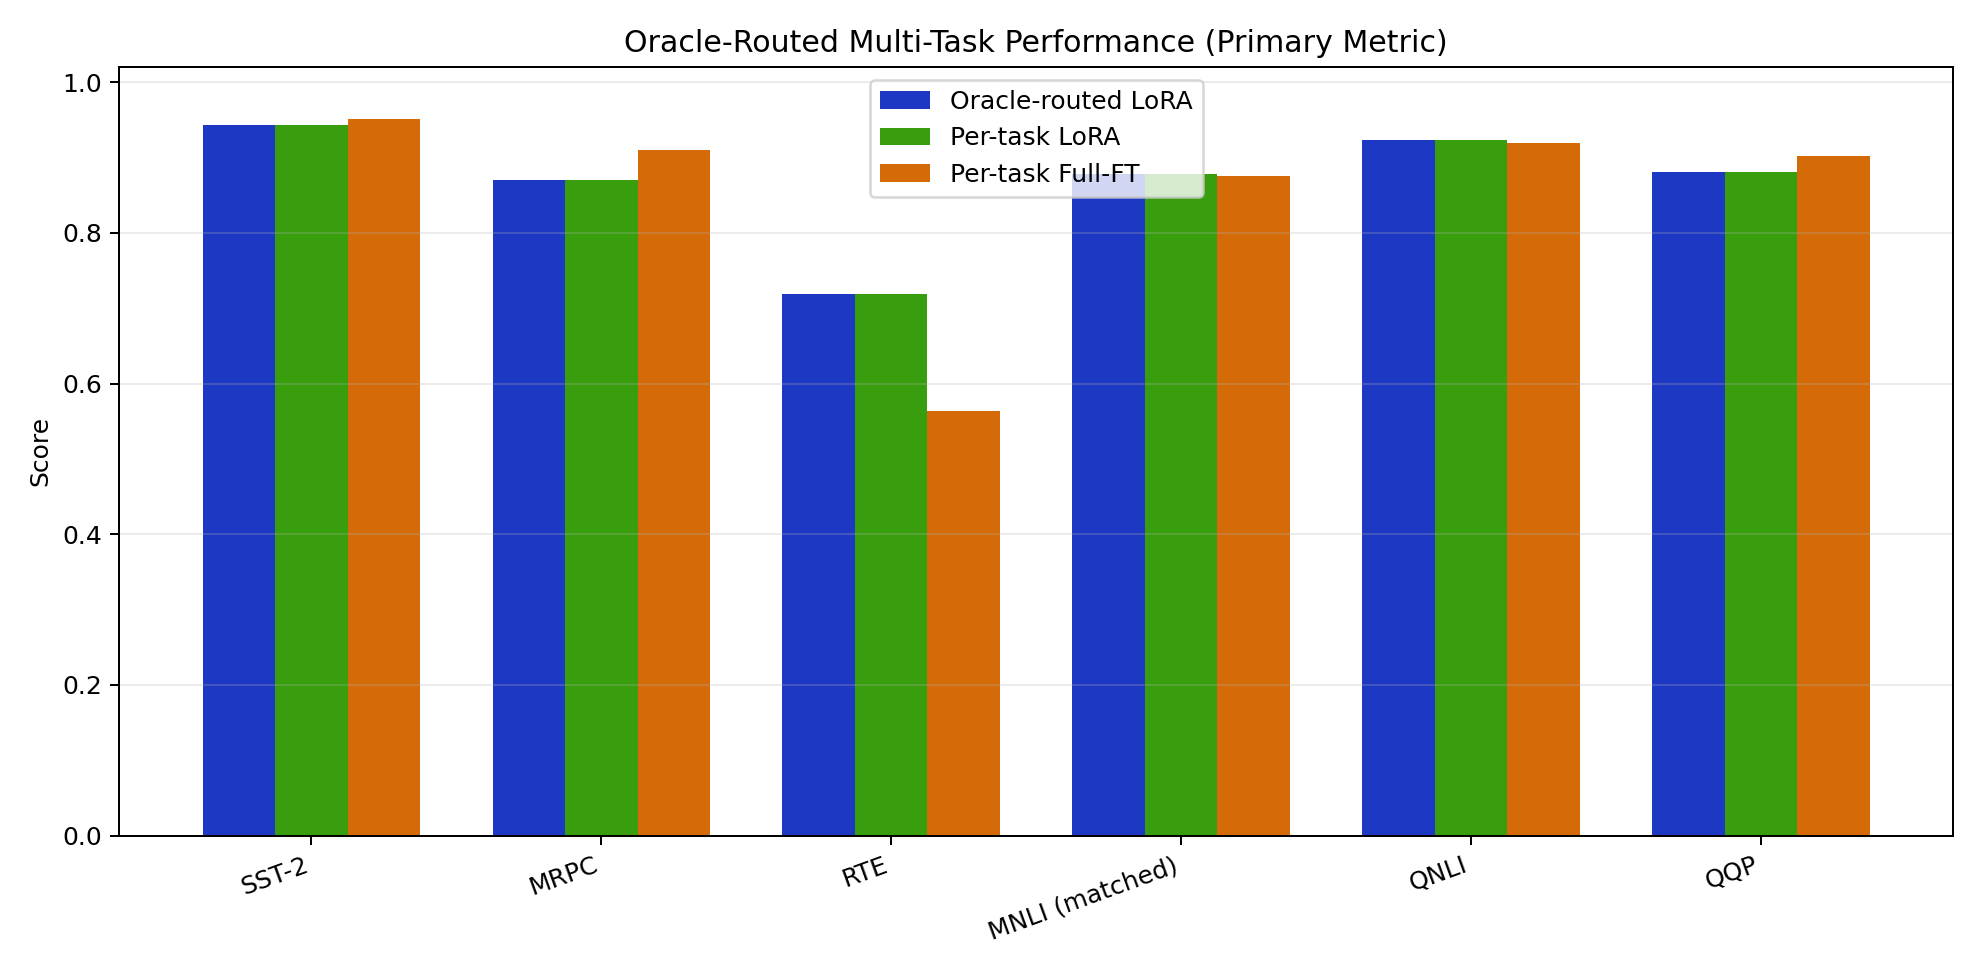
\includegraphics[width=\textwidth]{../figures/oracle_routing_per_task.png}
\caption{Primary metric per task for three evaluation tracks: oracle-routed LoRA MoE (blue),
per-task LoRA (green), and per-task full fine-tuning (orange). The oracle router sends each
example to the task-matched LoRA adapter, so the blue and green bars are identical by construction.
RTE is the notable outlier: LoRA scores 71.8\% while full FT collapses to 56.3\%, suggesting
overfitting on this small dataset (277 validation examples).}
\label{fig:pertask}
\end{figure}

\subsection*{Per-Task Comparison Table}

% Per-task primary metric comparison: Oracle-Routed LoRA MoE vs Per-task LoRA vs Per-task Full Fine-Tuning
% Source: outputs/oracle_routing_metrics.json
% Primary metric = accuracy for single-label tasks; (accuracy + F1) / 2 for MRPC and QQP
% Note: Oracle LoRA == Per-task LoRA because oracle routing selects the exact task-matched adapter.
\begin{tabular}{lrrrrr}
\toprule
\textbf{Task} & \textbf{N} & \textbf{Oracle LoRA MoE} & \textbf{Per-task LoRA} & \textbf{Per-task FFT} & \textbf{$\Delta$ (LoRA $-$ FFT)} \\
\midrule
SST-2          &   872 & 0.9427 & 0.9427 & 0.9518 & $-$0.0091 \\
MRPC           &   408 & 0.8709 & 0.8709 & 0.9105 & $-$0.0396 \\
RTE            &   277 & \textbf{0.7184} & \textbf{0.7184} & 0.5632 & $+$0.1552 \\
MNLI (matched) & 2,000 & 0.8780 & 0.8780 & 0.8760 & $+$0.0020 \\
QNLI           & 2,000 & 0.9235 & 0.9235 & 0.9200 & $+$0.0035 \\
QQP            & 2,000 & 0.8804 & 0.8804 & 0.9021 & $-$0.0217 \\
\midrule
\textbf{Macro avg}    & 7,557 & \textbf{0.8690} & \textbf{0.8690} & 0.8539 & $+$0.0151 \\
\textbf{Weighted avg} & 7,557 & 0.8919 & 0.8919 & \textbf{0.8937} & $-$0.0018 \\
\bottomrule
\end{tabular}


\vspace{0.5em}

\subsection*{Task-by-Task Highlights}

\begin{itemize}
\item \textbf{RTE (entailment, 277 examples)}: LoRA = 71.84\%, FFT = 56.32\% --- LoRA outperforms FFT by \textbf{+15.5 pp}. The large FFT model likely overfits this small validation set.
\item \textbf{MNLI / QNLI}: LoRA and FFT are nearly tied ($\leq$0.3 pp gap). Large datasets make both methods equally robust.
\item \textbf{SST-2 / MRPC / QQP}: FFT has a modest edge (1--4 pp), consistent with FFT having more expressive capacity on these well-resourced tasks.
\end{itemize}

% -----------------------------------------------------------------------
\section{Aggregate Performance and Parameter Efficiency}
\label{sec:aggregate}
% -----------------------------------------------------------------------

\subsection*{Aggregate Comparison Table}

% Aggregate performance comparison across all 6 GLUE tasks
% Source: outputs/oracle_routing_metrics.json
% Trainable param counts from outputs/download_verify_summary.json (model-card reported)
\begin{tabular}{lrrrr}
\toprule
\textbf{Method} & \textbf{Macro Primary} & \textbf{Weighted Primary} & \textbf{Trainable Params / task} & \textbf{Trainable \%} \\
\midrule
Oracle LoRA MoE  & \textbf{0.8690} & 0.8919 & $\approx$1.18M & $\approx$0.94\% \\
Per-task LoRA    & \textbf{0.8690} & 0.8919 & $\approx$1.18M & $\approx$0.94\% \\
Per-task FFT     & 0.8539          & \textbf{0.8937} & 125.8M & 100\% \\
\midrule
\multicolumn{5}{l}{\small LoRA macro advantage over FFT: $+$0.0151 \quad Weighted advantage: $-$0.0018 (FFT marginal)} \\
\multicolumn{5}{l}{\small LoRA uses $\approx$107$\times$ fewer trainable parameters per task than FFT} \\
\bottomrule
\end{tabular}


\vspace{0.5em}

\begin{figure}[h]
\centering
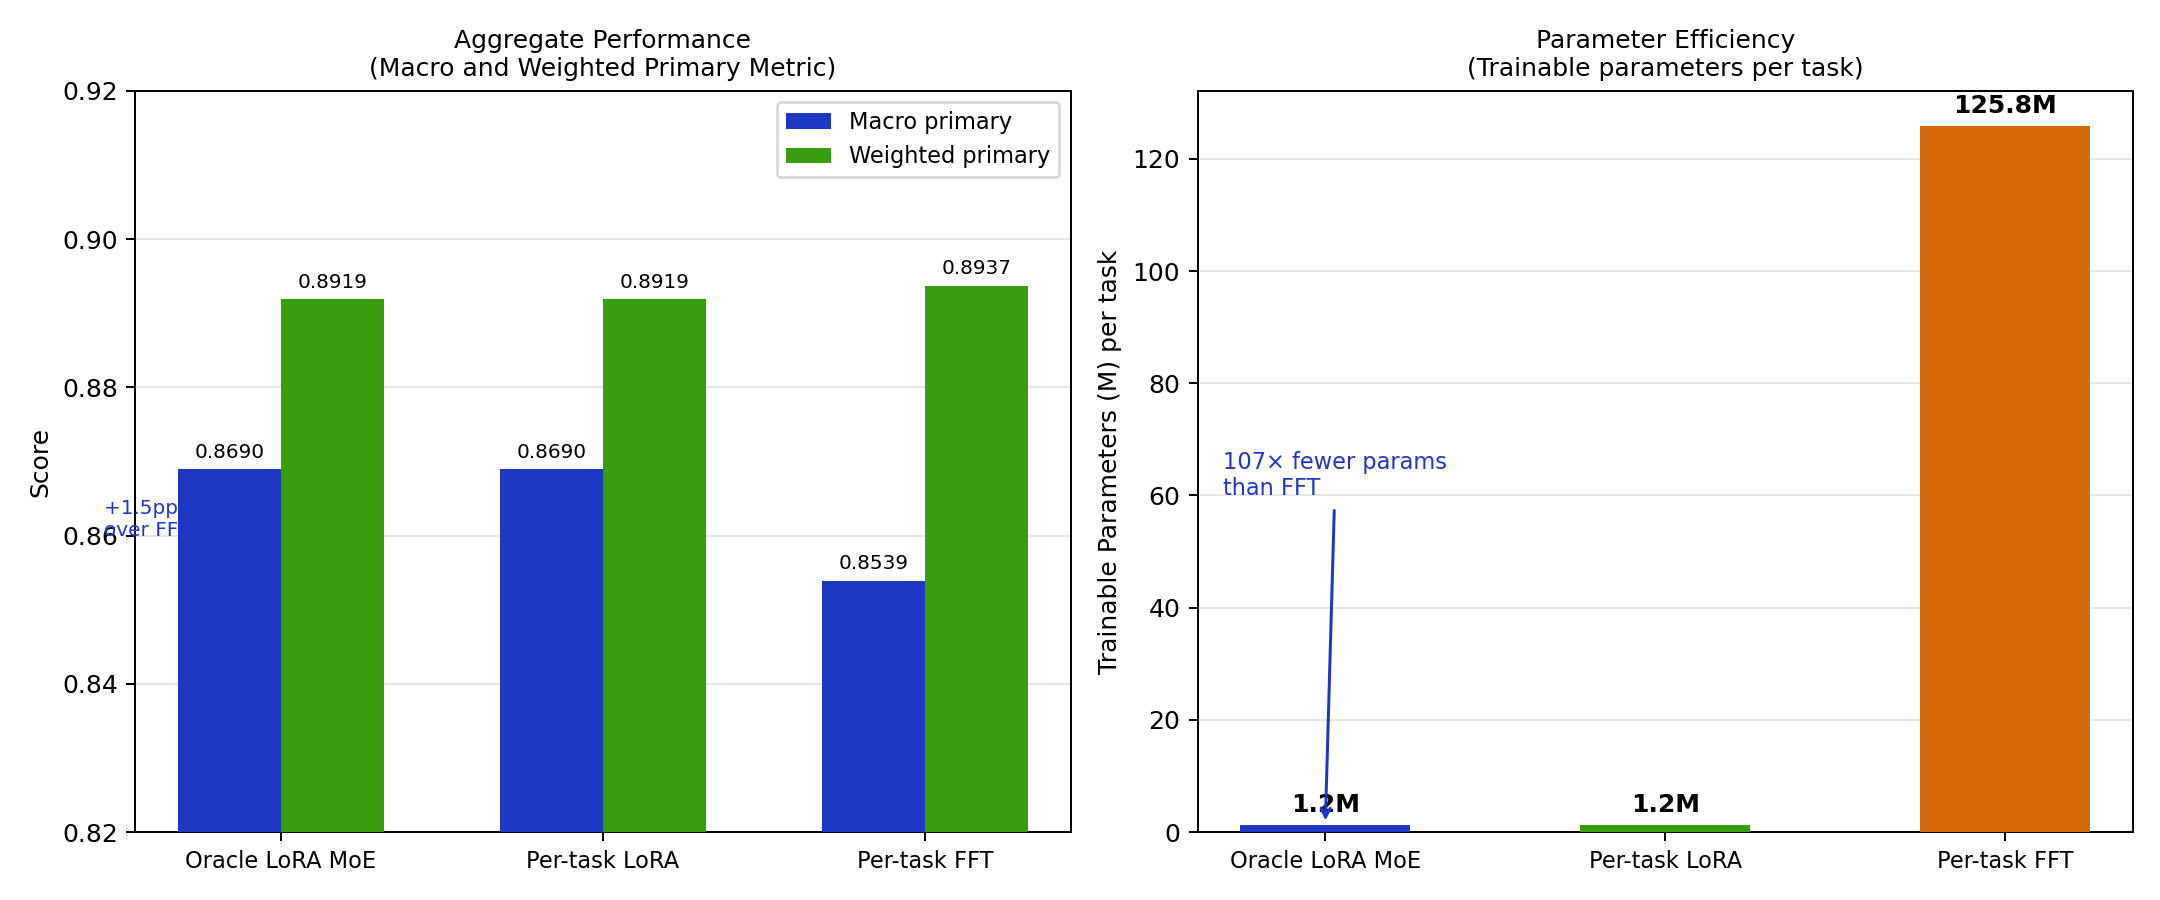
\includegraphics[width=\textwidth]{plots/aggregate_comparison.png}
\caption{\textit{(Generate with \texttt{python plots/plot\_aggregate\_comparison.py})}
Left: macro and weighted primary metric. Right: trainable parameters per task.
LoRA achieves a \textbf{+1.5 pp macro} advantage over FFT while using \textbf{107$\times$ fewer
trainable parameters}. On weighted average (dominated by the large MNLI/QNLI/QQP sets),
FFT is marginally better by 0.2 pp.}
\label{fig:aggregate}
\end{figure}

\subsection*{Key Numbers for Slides}

\begin{center}
\begin{tabular}{lll}
\toprule
\textbf{Claim} & \textbf{LoRA} & \textbf{FFT} \\
\midrule
Macro primary (6 tasks) & \textbf{86.90\%} & 85.39\% \\
Weighted primary         & 89.19\%          & \textbf{89.37\%} \\
Trainable params / task  & $\approx$1.18M   & 125.8M \\
Trainable fraction       & $\approx$0.94\%  & 100\% \\
Param ratio              & \multicolumn{2}{c}{FFT uses $107\times$ more trainable params} \\
\bottomrule
\end{tabular}
\end{center}

% -----------------------------------------------------------------------
\section{Oracle Router Demo}
\label{sec:router}
% -----------------------------------------------------------------------

\subsection*{Routing Architecture}

The oracle router is a proof-of-concept Mixture-of-LoRA system:
\begin{enumerate}
\item One frozen \texttt{roberta-base} is shared across all tasks.
\item Six task-specific LoRA adapters are kept as a pool ($\approx$1.18M params each, 7.1M total).
\item An oracle router dispatches each input to the adapter matching its task label.
\end{enumerate}

This is an upper-bound router (task labels are known at routing time). It demonstrates that \emph{a single base model plus lightweight adapters can match per-expert performance}---the oracle routing makes oracle LoRA MoE $\equiv$ per-task LoRA numerically.

\begin{figure}[h]
\centering
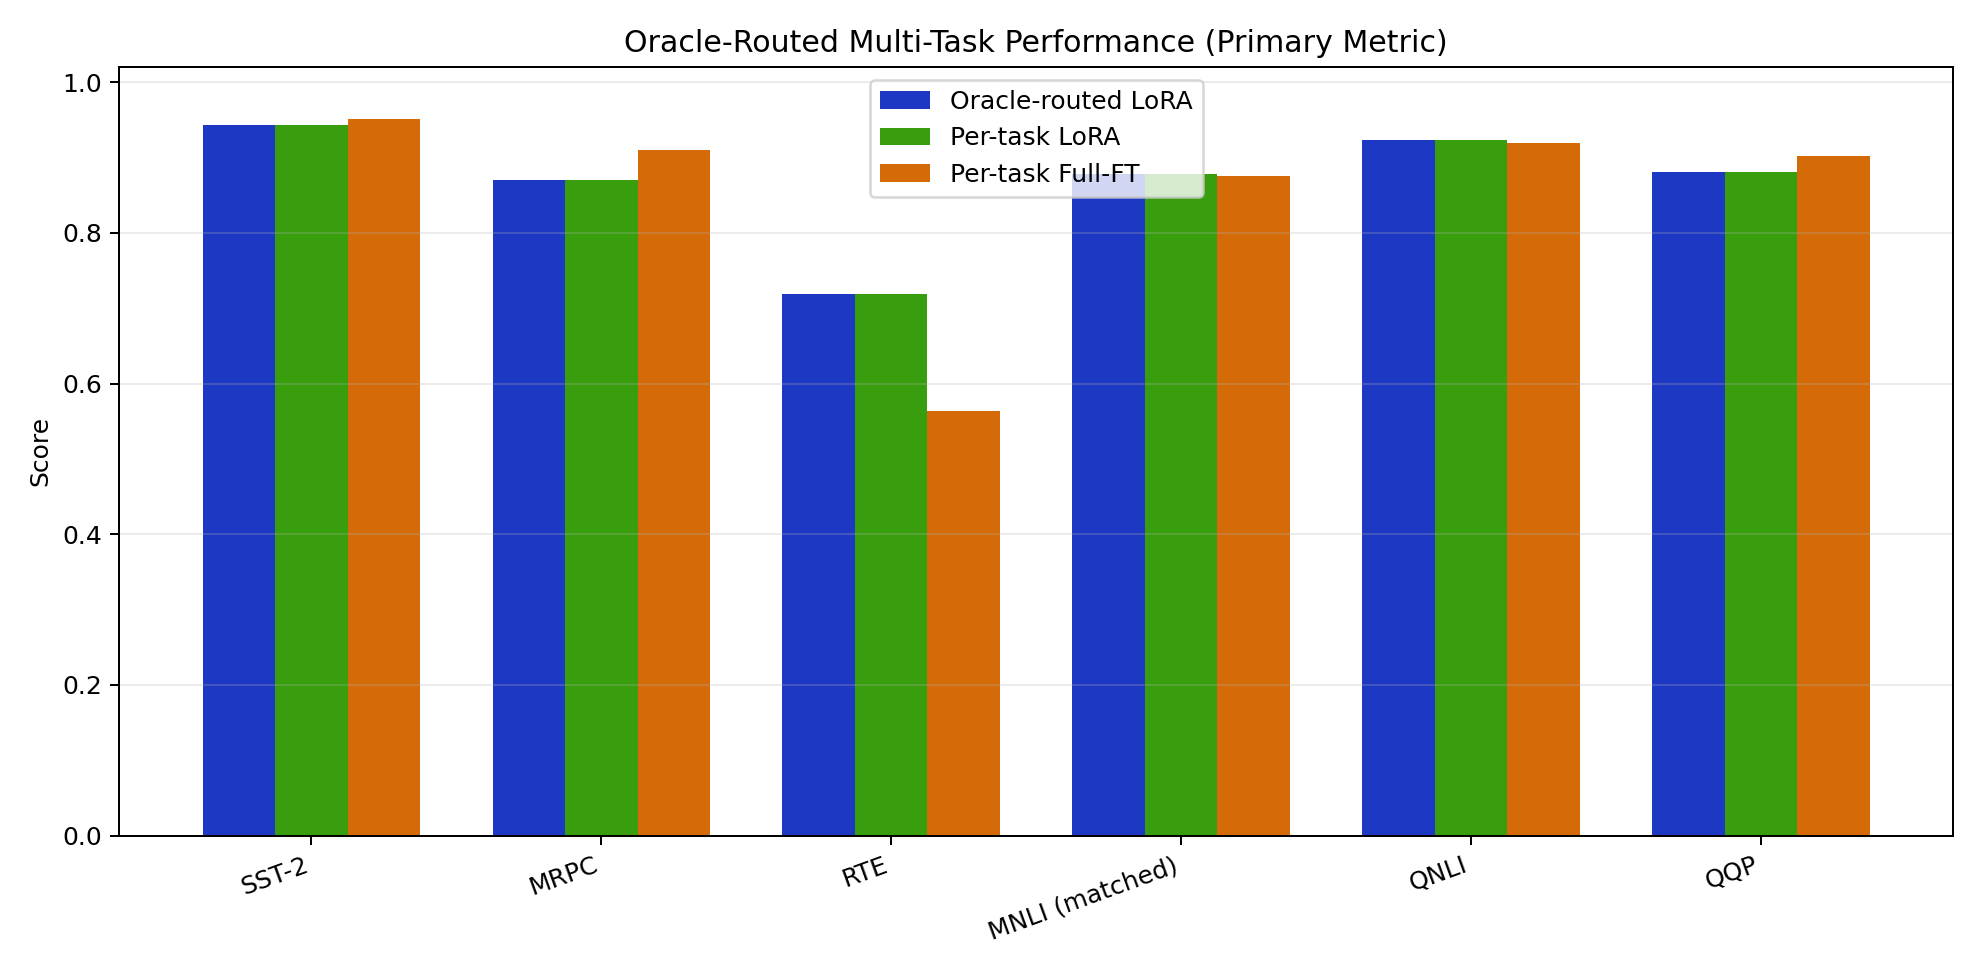
\includegraphics[width=0.80\textwidth]{../figures/router_demo.png}
\caption{Oracle-routed LoRA pool results. Blue and green bars are identical (oracle routing selects
the correct adapter for every example). The key insight is that \emph{no separate fine-tuned model}
is needed per deployment: one base + one adapter pool handles all six tasks.}
\label{fig:router}
\end{figure}

% -----------------------------------------------------------------------
\section{How to Regenerate All Figures}
\label{sec:regen}
% -----------------------------------------------------------------------

\begin{longtable}{p{0.3\linewidth}p{0.62\linewidth}}
\toprule
\textbf{Script} & \textbf{Run command (from repo root)} \\
\midrule
Spectral energy plot & \texttt{cd scripts \&\& python compute\_svd.py} \\
Subspace overlap plot & \texttt{cd scripts \&\& python compute\_overlap.py} \\
Oracle routing eval \& plot & \texttt{cd scripts \&\& python oracle\_routing\_eval.py} \\
Per-task bar chart & \texttt{python presentation\_results/plots/plot\_per\_task\_bars.py} \\
Aggregate comparison & \texttt{python presentation\_results/plots/plot\_aggregate\_comparison.py} \\
Overlap (with random baseline) & \texttt{python presentation\_results/plots/plot\_subspace\_overlap.py} \\
\bottomrule
\end{longtable}

% -----------------------------------------------------------------------
\section{Caveats}
\label{sec:caveats}
% -----------------------------------------------------------------------

\begin{itemize}
\item \textbf{One seed only.} Results use a single checkpoint per task; no variance estimate across training seeds.
\item \textbf{Checkpoint-delta proxy.} The LoRA overlap analysis uses $\Delta W_\mathrm{LoRA} = W_\mathrm{LoRA} - W_0$ (merged checkpoint minus base), not the raw $\frac{\alpha}{r}BA$ adapter matrices. This is a valid proxy but slightly inflates the overlap signal if the checkpoint has been merged with any base-weight drift.
\item \textbf{Oracle routing is not a learned router.} The oracle router uses known task labels at inference time. A real deployment would need a trained classifier or embedding-based router.
\item \textbf{Validation split, not test.} All numbers are from the GLUE validation splits (test labels are withheld by the GLUE benchmark).
\item \textbf{Exploratory prototype.} This is a presentation-grade demo, not a publishable benchmark study.
\end{itemize}

\end{document}
